\documentclass[9pt]{article}

\usepackage{amssymb}
\usepackage{amsmath}
\usepackage{amsfonts}
\usepackage{comment}
\usepackage{fancyhdr}
\usepackage{mathrsfs}
\usepackage{enumitem}
\usepackage{graphicx}

\usepackage{tikz}

\voffset = -50pt
%\textheight = 700pt
\addtolength{\textwidth}{60pt}
\addtolength{\evensidemargin}{-30pt}
\addtolength{\oddsidemargin}{-30pt}
%\setlength{\headheight}{44pt}

\newcommand{\qed}{\hfill \ensuremath{\Box}}


\newcommand*\circled[1]{\tikz[baseline=(char.base)]{
            \node[shape=circle,draw,inner sep=2pt] (char) {#1};}}

\newcommand{\Z}{\mathbb{Z}}
\newcommand{\I}{\mathbb{I}}
\newcommand{\M}{\mathbb{M}}
\newcommand{\R}{\mathbb{R}}
\newcommand{\C}{\mathbb{C}}
%\setcounter{section}{-1}

\begin{document}
\topskip0pt
\vspace*{\fill}
\begin{center}
{\Huge \begin{tabular}{@{}ll@{}}
   Class: & CECS 201, Section 7 \\ \\ \\
   Lab: & 7 \\ \\ \\
   Title: & 7 Segment Decoder \\ \\ \\
   Student Name: & Barry Joseph Okonoboh \\ \\ \\
   Due Date: & 11:59:59 P.M., 23, March 2015 \\ \\ \\
   Instructor: & Dan Cregg
\end{tabular}}
\end{center}
\vspace*{\fill}
\newpage
\begin{enumerate}
%%%%%%%%%%%%%%%%%%%%%%%%%%%%%%%%%%%%%%%%01%%%%%%%%%%%%%%%%%%%%%%%%%%%%%%%%%%%%%%
   \item[b.] \textbf{Introduction.} This lab involves using logic gates to
               determine if a four bit unsigned number is a prime.
   \item[c.] \textbf{Project Description.} The four bits of the number are
             mapped to four inputs $A$, $B$, $C$ and $D$. If the number
             represented by the bits is true, then the output is 1; otherwise,
             it is 0. A Karnaugh map is used to simplify the equation and both
             the simplified and unsimplified equations are simultaneously tested
             using the Diligent board.
  	\item[d.] \textbf{Schematic.}
             \begin{center}
                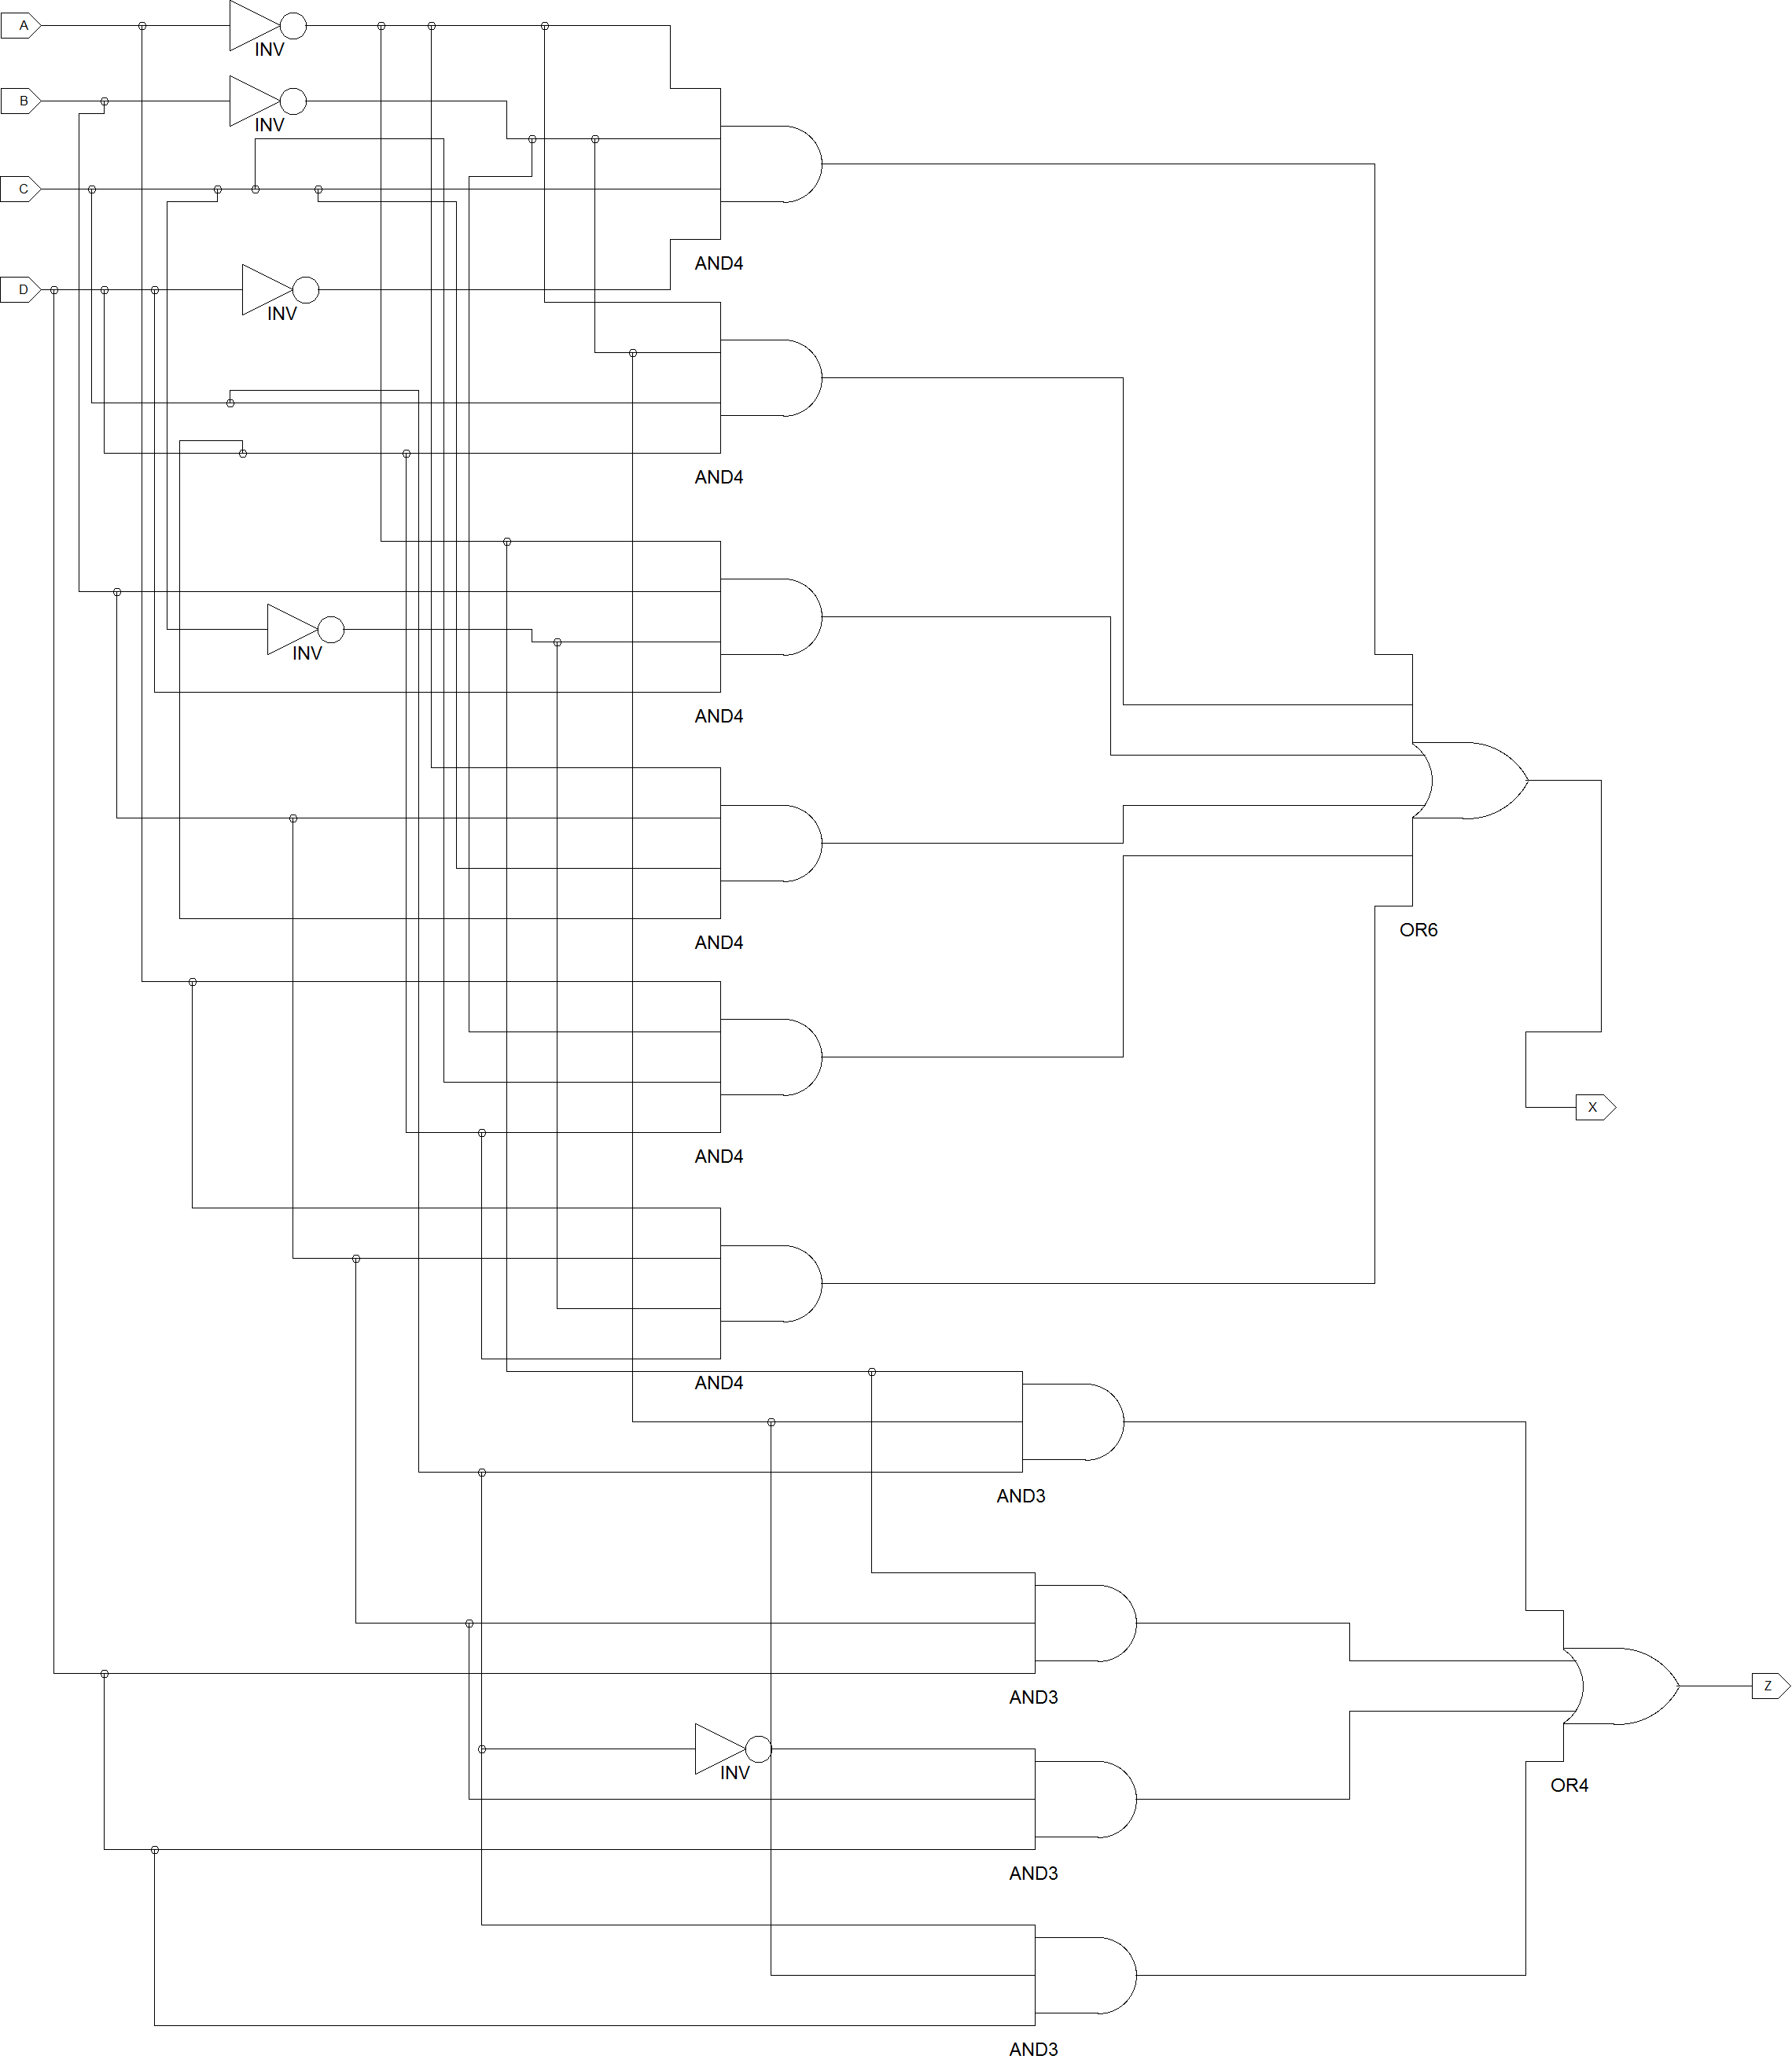
\includegraphics[width=\textwidth]{schematic.png}
             \end{center}
             
             \textbf{Truth Table.}   
   
   \begin{center}
    \begin{tabular}{@{}|c|c|c|c|c|c|c|c|c|c|c|c|@{}}
   \hline
         $A$ & $B$ & $C$ & $D$ & ledA & ledB & ledC & ledD & ledE & ledF & ledG
             & ledEnable \\ \hline
         0 & 0 & 0 & 0 & 0 & 0 & 0 & 0 & 0 & 0 & 1 & 1 \\ \hline
         0 & 0 & 0 & 1 & 1 & 0 & 0 & 1 & 1 & 1 & 1 & 0 \\ \hline
         0 & 0 & 1 & 0 & 0 & 0 & 1 & 0 & 0 & 1 & 0 & 0 \\ \hline
         0 & 0 & 1 & 1 & 0 & 0 & 0 & 0 & 1 & 1 & 0 & 0 \\ \hline
         0 & 1 & 0 & 0 & 1 & 0 & 0 & 1 & 1 & 0 & 0 & 0 \\ \hline
         0 & 1 & 0 & 1 & 0 & 1 & 0 & 0 & 1 & 0 & 0 & 0 \\ \hline
         0 & 1 & 1 & 0 & 0 & 1 & 0 & 0 & 0 & 0 & 0 & 0 \\ \hline
         0 & 1 & 1 & 1 & 0 & 0 & 0 & 1 & 1 & 1 & 1 & 0 \\ \hline
         1 & 0 & 0 & 0 & 0 & 0 & 0 & 0 & 0 & 0 & 0 & 0 \\ \hline
         1 & 0 & 0 & 1 & 0 & 0 & 0 & 0 & 1 & 0 & 0 & 0 \\ \hline
         1 & 0 & 1 & 0 & 0 & 0 & 0 & 1 & 0 & 0 & 0 & 0 \\ \hline
         1 & 0 & 1 & 1 & 1 & 1 & 0 & 0 & 0 & 0 & 0 & 0 \\ \hline
         1 & 1 & 0 & 0 & 0 & 1 & 1 & 0 & 0 & 0 & 1 & 0 \\ \hline
         1 & 1 & 0 & 1 & 1 & 0 & 0 & 0 & 0 & 1 & 0 & 0 \\ \hline
         1 & 1 & 1 & 0 & 0 & 1 & 1 & 0 & 0 & 0 & 0 & 0 \\ \hline
         1 & 1 & 1 & 1 & 0 & 1 & 1 & 1 & 0 & 0 & 0 & 0 \\ \hline
\end{tabular}
   \end{center}
\end{enumerate}
\end{document}